\documentclass[xcolor=table]{beamer}

% -----------General Settings ------------
\usetheme{default}
\usetheme{Antibes}
\usecolortheme{dolphin}
\setbeamercolor{normal text}{bg=blue!3}
\beamertemplatetransparentcovereddynamicmedium
\beamertemplateshadingbackground{blue!4}{black!8}
\graphicspath{{./images/}} %images path
\title[Image Processing to Detect Worms]{Image Processing to Detect Worms}
\author[Javier Fern\'andez]{Javier Fern\'andez}
\institute[Uppsala University]{Uppsala University. Uppsala, Sweden}

\begin{document}
\maketitle

%----------- Introduction ----------------

\section{Introduction}
\subsection{C.elegans}

\begin{frame}{Caenorhabditis elegans (C.elegans)}

\begin{itemize}
\item Widely used organism
\item Model system for biological process such as: inmunity,
  behavior and metabolism
\item High-throughput screening (HTS) of C.elegans is used to identify
  promising drugs and regulators.
\end{itemize}

\end{frame}

\subsection{The problem}
\begin{frame}{The Problem: Motivation and Purpose}
\begin{itemize}
\item The deployment in HTS has been limited to long and intensive manual assays.
\item Many scientific questions require measurements on individual worms.
\item Worms identification should be automatic
\end{itemize}

\end{frame}

\subsection{Background}
\begin{frame}{Background on Worm Detection}

\begin{itemize}
  \item Methods base on worm locomotion. Exploit motion cues and 
    cannot be used in still images of high-throughput screens. \pause
  \item Few methods attempt to overcome worm interaction and none
    solves it successfully. \pause
  \item Most methods use an initial strategy involving: Segmentation,
    Skeletonization and Shape Parameterization.
\end{itemize}

\end{frame}

% -----------------------------------------

\subsection{Objectives}
\begin{frame}{Objectives}
\vskip10pt

\large \textbf{General Objective}\\
\vskip7pt

\begin{itemize}
  \item To design and implement an image processing methodology 
to detect and fit the shape of worms in digital images
\end{itemize}

\end{frame}

\begin{frame}{Objectives}
\pause \large \textbf{Specific Objectives}\\
\vskip7pt

\begin{itemize}
  \item To design an algorithm based on image processing techniques that 
receives images of worms in liquid culture as input, and outputs fitted
 shapes of these worms.\pause
 \begin{itemize}
 \item To review the background on image segmentation techniques. \pause
 \item To design a shape descriptor and a rasterization method to 
   represent worms in numerical terms.\pause
 \item To review the background on shape matching and object recognition and
propose a matching approach.
 \end{itemize}
\pause 
\item To implement the designed algorithm as a plugin for Endrov
\end{itemize}

\end{frame}

%-----------------------------------------

\section{Methodology}
\begin{frame}{}
\begin{center}
\LARGE METHODOLOGY
\end{center}
\end{frame}


\subsection{Solution Methodology Flowchart}
\begin{frame}{}

\begin{figure}[h t b p ! H]
 \centering
   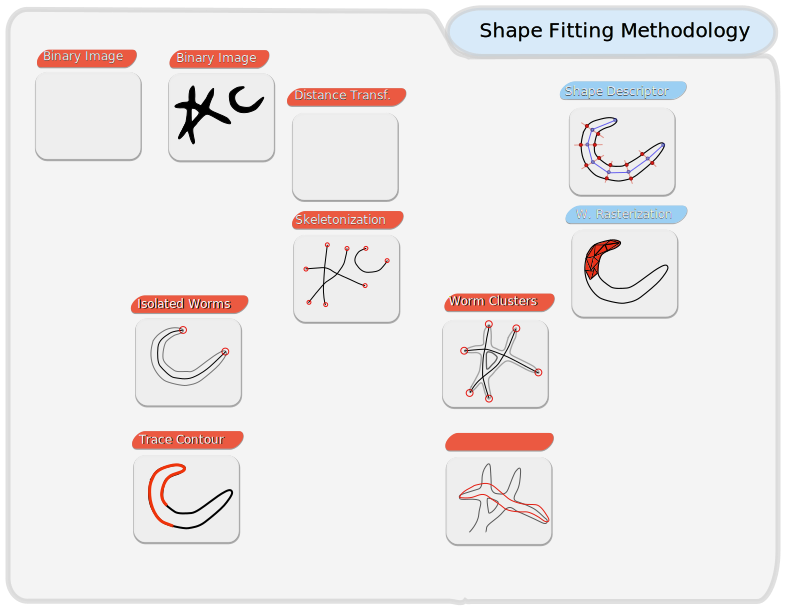
\includegraphics[scale=0.46]{diagrams/design.pdf}
\end{figure}
\end{frame}


% -------- Original and Thresholding -----------

\subsection{Thresholding}
\begin{frame}{Thresholding}

\begin{columns}[c]
\column{1.5in}
\includegraphics[scale=0.27]{original}
\column{1.5in}
\includegraphics[scale=0.27]{thres/worms}

\end{columns}

\end{frame}

% -------- Distance Transformation  -----------

\subsection{Distance Transformation}
\begin{frame}{Distance Transformation: Manhattan Distance}

\begin{columns}[c]
\column{2.4in}
\begin{itemize}
\item Improve skeletonization algorithm \pause
\item Trace contour of isolated worms \pause
\item Automatic calculation of worm profile \pause
\item Path guessing algorithm
\end{itemize}
\column{2in}
\includegraphics[scale=0.27]{results/test1/dt-shape1}

\end{columns}

\end{frame}


% -------- Skeletonization  -----------

\subsection{Skeletonization}
\begin{frame}{Worm Skeletonization}

\begin{columns}[c]
\column{2.4in}
\begin{itemize}
\item Thinning Algorithm $+$ Distance Map \pause
\item 1 pixel thick paths that tend to the medial axes \pause
\item Skeleton endpoint expansion and Worm Endpoint detection \pause
\item Segmentation in groups
\end{itemize}
\column{2in}
\includegraphics[scale=0.3]{skeleton1}

\end{columns}

\end{frame}


% -------- Shape Matching  -----------

\subsection{Shape Matching}
\begin{frame}{Isolated Worms}

\begin{columns}[c]
\column{2.4in}
\begin{itemize}
\item Contour can be traced easily.The shape is rasterized 
and thus fitted \pause
\item Worm Profiling 
\end{itemize}
\column{2.2in}
\includegraphics[scale=0.5]{iso}
\end{columns}

\end{frame}

% -------- Shape Matching  -----------

\subsection{Shape Matching}
\begin{frame}{Worm Cluster: Matching Approach}

\begin{columns}[c]
\column{2.6in}
\begin{itemize}
\item Calculate feasible worm paths from every endpoint
  \begin{itemize}
  \item Paths no longer than 1.5 of the average worm size
  \item Path guessing algorithm 
  \end{itemize}
\pause\item A worm shape is constructed given a path and a worm
  profile \pause
\item The shape is deformed until the best possible match is
  found \pause
\item For this is required: a shape descriptor, a
  rasterization method, distance measure between shapes
  and a optimization approach.
\end{itemize}
\column{2.2in}
\includegraphics[scale=0.3]{clusterskeleton}
\end{columns}

\end{frame}


% -------- Shape Matching  -----------

\subsection{Shape Matching}
\begin{frame}{Worm Shape Descriptor}

\begin{columns}[c]
\column{2.0in}
\begin{itemize}
\item Set of control points connected by straight lines \pause
\item Bisectors of control point angles \pause
\item Calculate contour points from the worm profile \pause
\item Trace the contour through a Cardinal Spline \\
\item The shape is rasterized by triangulating the area and 
  rasterizing each triangle individually.
\end{itemize}
\column{2.3in}
\includegraphics<1>[scale=0.45]{control}
\includegraphics<2>[scale=0.45]{bisec}
\includegraphics<3>[scale=0.45]{prof}
\includegraphics<4->[scale=0.45]{shape}
\end{columns}

\end{frame}

% -------- Shape Matching  -----------

\subsection{Shape Matching}
\begin{frame}{Matching Optimization}

  \begin{itemize}
  \item A worm shape is generated given a skeleton path \pause
  \item The shape is deformed until the distance between the shape and the image 
    is minimized, thus obtaining a worm conformation. \pause
  \item The distance is measured through an Energy Formulation defined as the
    sum of the External and Internal energy. \pause
    \begin{itemize}
    \item External: How well the model matches the data \pause
    \item Internal: Model resistance to be pushed into not coherent directions
    \end{itemize}\pause
  \item The best set of conformations is chosen: maximizing the amount of covered
    endpoints and minimizing the total energy \pause
  \item Incorrect conformations can be easily fixed manually
  \end{itemize}

\end{frame}

%---------------- Results ---------------

\section{Results}
\begin{frame}{}
\begin{center}
\LARGE RESULTS
\end{center}
\end{frame}

\subsection{Test Set}
\begin{frame}{Test Set: test Image 1}

  \begin{itemize}
  \item Images in increasing difficulty level: number of worms
    and overlaps
  \end{itemize}

\begin{table}[h]
\begin{center}
\begin{tabular}[h]{|c|c|c|c|c|}
    \hline
    \rowcolor{gray!35}
    Test & Isolated & Clusters & Clustered Worms & Total\\
    Test 1 & 11/19 (57.8\%) & 3 & 8/19 (42.1\%) & 19 \\
    \hline
  \end{tabular}
\end{center}
\end{table}

\begin{center}
\includegraphics[scale=0.25]{results/test1/original}
\end{center}

\end{frame}

\begin{frame}{Test Set: test Image 2}

  \begin{itemize}
  \item Images in increasing difficulty level: number of worms
    and overlaps
  \end{itemize}

\begin{table}[h]
\begin{center}
\begin{tabular}[h]{|c|c|c|c|c|}
    \hline
    \rowcolor{gray!35}
    Test & Isolated & Clusters & Clustered Worms & Total\\
    Test 2 & 8/33 (24.2\%) & 3 & 25/33 (75.7\%)& 33 \\    
    \hline
  \end{tabular}
\end{center}
\end{table}


\begin{center}
\includegraphics[scale=0.22]{results/test2/original2}
\end{center}

\end{frame}

\begin{frame}{Test Set: test Image 3}

  \begin{itemize}
  \item Images in increasing difficulty level: number of worms
    and overlaps
  \end{itemize}

\begin{table}[h]
\begin{center}
\begin{tabular}[h]{|c|c|c|c|c|}
    \hline
    \rowcolor{gray!35}
    Test & Isolated & Clusters & Clustered Worms & Total\\
    Test 3 & 13/38 (34.2\%)& 5 & 25/38 (65.7\%) & 38 \\
    \hline
  \end{tabular}
\end{center}
\end{table}

\begin{center}
\includegraphics[scale=0.25]{results/test3/original3}
\end{center}
\end{frame}



% ------ Matching Results ------

\subsection{Matching Results}
\begin{frame}{Matching Experiments}

  \begin{itemize}
  \item Automated matching. 
    \begin{itemize}
    \item Two different path sets: With and without Path Guessing 
    \item Missing endpoints 
    \end{itemize}
  \item Manual Adjustment
    \begin{itemize}
    \item The incorrectly assigned conformations are fixed following
      a manual process
    \end{itemize}
    
  \end{itemize}
  

\end{frame}

\begin{frame}{Matching Results: Test Image 1}

\large \textbf{Automated Matching}
\begin{scriptsize}
\begin{table}[h]
\begin{center}
\begin{tabular}[h]{|c|c|c|c|c|}
    \hline
    \rowcolor{gray!35}
    Path finding & Iso. Matching & Cluster Matching 
    & Total
    & Time (s) \\
    Every Path & 11/11 (100\%) & 6/8 (75\%) & 17/19 (\alert{89.5\%})& 6.47 \\
    \hline
    P.Guessing & 11/11 (100\%) & 8/8 (100\%) & 19/19 (\alert{100\%}) & 7.53 \\     
    \hline  
  \end{tabular}
\end{center}
\end{table}
\end{scriptsize} 
\end{frame}


\begin{frame}{Matching Results: Test Image 2}

\large \textbf{Automated Matching}
\begin{scriptsize}
\begin{table}[h]
\begin{center}
\begin{tabular}[h]{|c|c|c|c|c|}
    \hline
    \rowcolor{gray!35}
    Path finding & Iso. Matching & Cluster Matching 
    & Total
    & Time (s) \\ 
    Every Path - me & 8/8 (100\%) & 7/25 (28\%) & 15/33 (\alert{45.4\%}) & 21.8  \\ 
    \hline
    P.Guessing - me & 8/8 (100\%) & 10/25 (40\%) & 18/33 (\alert{54.5\%}) & 23.7 \pause \\
    \hline
    Every Path + me & 8/8 (100\%)& 15/23 (65.2\%) & 23/33 (\alert{69.7\%})& 42.3 \\
    \hline
    P.Guessing + me & 8/8 (100\%)& 21/25 (84\%) & 29/33 (\alert{87.8\%}) & 45 \\
    \hline
  \end{tabular}
\end{center}
\end{table}
\end{scriptsize}\pause

\large \textbf{Manual Adjustment}\\ \vskip10pt
  After 4 operations the final matching percentage increases from 87.8\%
  to 100\%
\end{frame}

\begin{frame}{Matching Results: Test Image 3}

\large \textbf{Automated Matching}
\begin{scriptsize}
\begin{table}[h]
\begin{center}
\begin{tabular}[h]{|c|c|c|c|c|}
    \hline
    \rowcolor{gray!35}
    Path finding & Iso. Matching & Cluster Matching 
    & Total
    & Time (s) \\ 
   Every Path - me & 13/13 (100\%) & 5/25 (20\%) & 18/38 (\alert{47.3\%}) & 26.4 \\ 
    \hline
    P.Guessing - me & 13/13 (100\%) & 7/25 (28\%) & 20/38 (\alert{52.6\%}) & 28.7 \pause\\
    \hline
    Every Path + me & 13/13 (100\%)& 13/25 (52\%) & 26/38 (\alert{68.4\%})& 36.2 \\
    \hline
    P.Guessing + me & 13/13 (100\%)& 16/25 (64\%) & 29/38 (\alert{76.3\%}) & 39.8 \\  
    \hline  
    \end{tabular}
\end{center}
\end{table}
\end{scriptsize} \pause

\large \textbf{Manual Adjustment}\\ \vskip10pt
  After 9 operations the final matching percentage increases from 76.3\% 
  to 100\%

\end{frame}

\subsection{Global Results: Best Matches}
\begin{frame}{Global Results: Best Matches}

\begin{table}[h]
\begin{center}
\begin{tabular}[h]{|c|c|c|}
    \hline
    \rowcolor{gray!35}
    Test Image & Automated Matching & After Manual Adjustment\\
    Image 1 & 100\% & 100\% \\
    Image 2 & 87.8\% & 100\% \\
    Image 3 & 76.3\% & 100\% \\
    \hline
    \end{tabular}
\end{center}
\end{table}
\end{frame}

\begin{frame}{Best automated and fixed matched on Test Image 2}
\begin{columns}[c]
\column{2.3in}
\includegraphics[scale=0.4]{results/test2/guessing-nobgframe}
\column{2.3in}
\includegraphics[scale=0.4]{results/test2/frame2-allnobg}
\end{columns}

\end{frame}

\subsection{Matching Energy}
\begin{frame}{Distribution of Matching Energy}
Energy values for the best three conformations starting from a set of
endpoints
\begin{figure}[htp]
    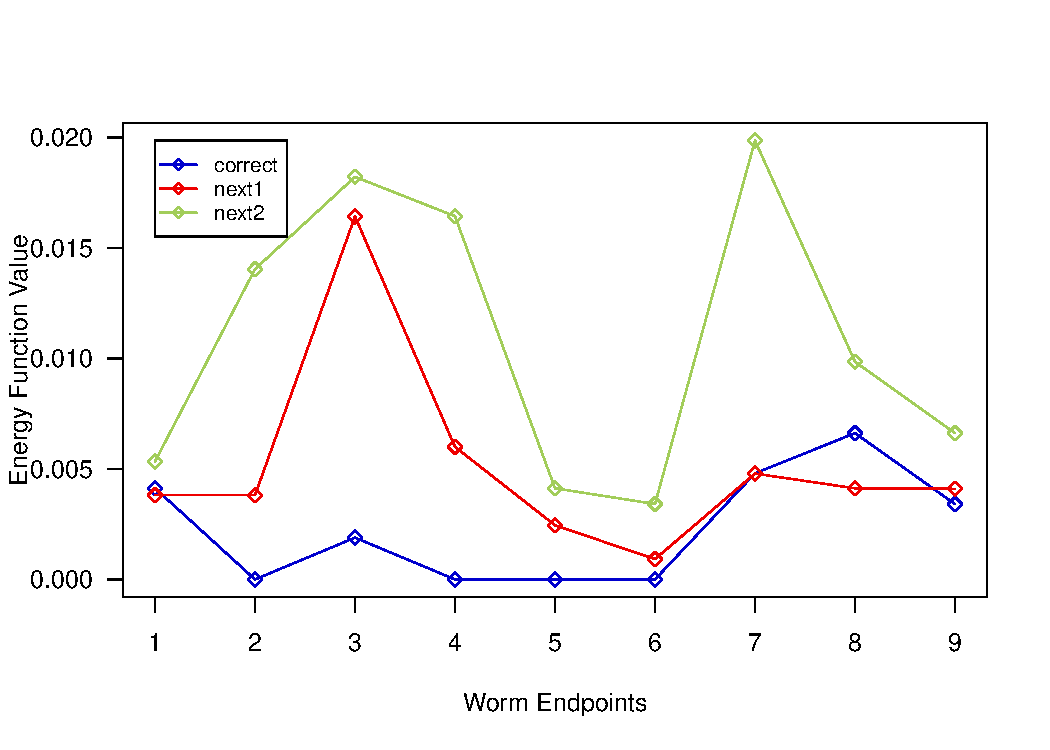
\includegraphics[scale=0.5]{results/test2/energy-graph}
 \end{figure}
\end{frame}

\begin{frame}{Distribution of Matching Energy}
\begin{itemize}
\item In the 75\% of the cases the best conformation results to be have
the lowest energy value \pause
\item The energy difference between the best and second best conformation in the other 
  25\% of the cases is very low. \pause
\item The correct conformation is always one of the top two
\end{itemize}
 \vskip6pt

\pause A more sophisticated objective function could tackle these differences, thus providing
better matching results.
\end{frame}

\section{Conclusions}
\begin{frame}{Conclusions}

\textbf{Solution Methodology}
  \begin{itemize}
  \item Feasible semi-automatic solution to detect
    and fit worm shapes \pause
  \item Time cost and matching accuracy is improved
    with respect to manual identification \pause
  \item An optimal match can be obtained through
    manual adjustments \pause
  \item The shape matching step is the most
    time consuming process \pause
  \item The methodology could be successfully
    implemented for Endrov
  \end{itemize}

\end{frame}

\begin{frame}{Conclusions}
\textbf{Isolated Worms}
  \begin{itemize}
  \item Isolated worms are totally identified in
    each case \pause
  \item An accurate worm profile can be calculated
    \end{itemize}
    
\pause \textbf{Worm Clusters}
\begin{itemize}
  \item The totality of endpoints must be detected.
    Manual adjustments are usually required \pause
  \item The shapes of the assigned conformations 
    represent accurately the worms in the image
  \end{itemize}

\end{frame}


\begin{frame}{Conclusions}
\textbf{Optimization}
  \begin{itemize}
  \item Path guessing algorithm improves 
    the matching accuracy considerably \pause
  \item The implemented local search is fast and 
    effective \pause
  \item The energy formulation is sensitive enough
    to provide correct conformations in the majority
    of the cases
  \end{itemize}

\end{frame}

\section{Future Work}
\begin{frame}{Future Work}

  \begin{itemize}
  \item Energy Formulation: A more
    sophisticated formulation \pause
  \item Endpoint Detection: Automated detection 
    of endpoints \pause
  \item Worm Trackers: Couple with worm
    trackers to provide optimal matches
    for individual images \pause
  \item Conformation Assignment: Improve the
    model (e.g. Non Bipartite Assignment
  \end{itemize}
\end{frame}

\section{Future Work}
\begin{frame}
\begin{center}
\LARGE Thanks for your attention
\end{center}

\end{frame}


\end{document}